\section{Git Branching and Merging}

\subsection{Objective}
The objective of this assignment was to demonstrate proficiency in Git branching, merging, and conflict resolution using the GitHub Desktop application.

\subsection{Steps Taken}

\subsubsection{Create a New Repository}
I opened GitHub Desktop and created a new repository called \texttt{git-advanced}.

\subsubsection{Clone the Repository}
Cloned the repository to my local machine by selecting the repository and clicking on the "Clone" button.

\subsubsection{Create and Switch to New Branch}
I created a new branch called \texttt{feature-1} by clicking on the "Current Branch" dropdown and selecting "New Branch."

\subsubsection{Create and Edit File}
I created a new file called \texttt{shared.txt} in my text editor with the following content:
\begin{verbatim}
This is a shared file.
Line 1: Original text.
Line 2: Original text.
\end{verbatim}

\subsubsection{Stage and Commit the File}
In GitHub Desktop, I staged the file by checking the box next to \texttt{shared.txt} and added a meaningful commit message before clicking the "Commit to feature-1" button.

\subsubsection{Push the Branch to GitHub}
I pushed the \texttt{feature-1} branch to GitHub by clicking on the "Push origin" button in the top-right corner.

\subsubsection{Create Another Branch}
I created another branch called \texttt{feature-2} using the same method as before: by selecting "New Branch" from the "Current Branch" dropdown.

\subsubsection{Checkout File from Main Branch}
I returned to the main branch and checked out the \texttt{shared.txt} file to ensure I had the original version.

\subsubsection{Modify the File}
I modified the \texttt{shared.txt} file to change the second line to:
\begin{verbatim}
Line 2: Modified text in feature-2.
\end{verbatim}

\subsubsection{Stage and Commit Changes}
In GitHub Desktop, I staged the changes and committed them with a meaningful message.

\subsubsection{Push the Branch to GitHub}
I pushed the \texttt{feature-2} branch to GitHub using the "Push origin" button.

\subsubsection{Switch Back to Feature-1}
I switched back to the \texttt{feature-1} branch by selecting it from the "Current Branch" dropdown.

\subsubsection{Modify the File Again}
I modified the \texttt{shared.txt} file again, changing the second line to:
\begin{verbatim}
Line 2: Modified text in feature-1.
\end{verbatim}

\subsubsection{Stage and Commit the Changes}
I staged and committed the changes in GitHub Desktop with a meaningful message.

\subsubsection{Push the Branch to GitHub}
I pushed the \texttt{feature-1} branch to GitHub.

\subsubsection{Merge Feature-1 into Main}
I merged \texttt{feature-1} into the main branch by switching to the main branch and using the "Merge into Current Branch" option.

\subsubsection{Merge Feature-2 into Main}
I then attempted to merge \texttt{feature-2} into the main branch, which introduced a conflict.

\subsubsection{Resolve the Conflict}
I resolved the conflict by editing \texttt{shared.txt} directly in my text editor, and then committed the resolution in GitHub Desktop.

\subsubsection{Push the Updated Main Branch}
I pushed the updated main branch to GitHub using the "Push origin" button.

\subsubsection{Delete the Feature Branches}
Finally, I deleted the \texttt{feature-1} and \texttt{feature-2} branches from the repository in GitHub Desktop.

\subsection{Deliverables}
The final submission includes:
\begin{itemize}
    \item A screenshot of the GitHub repository showing the commit history and branching.
    \begin{center}
        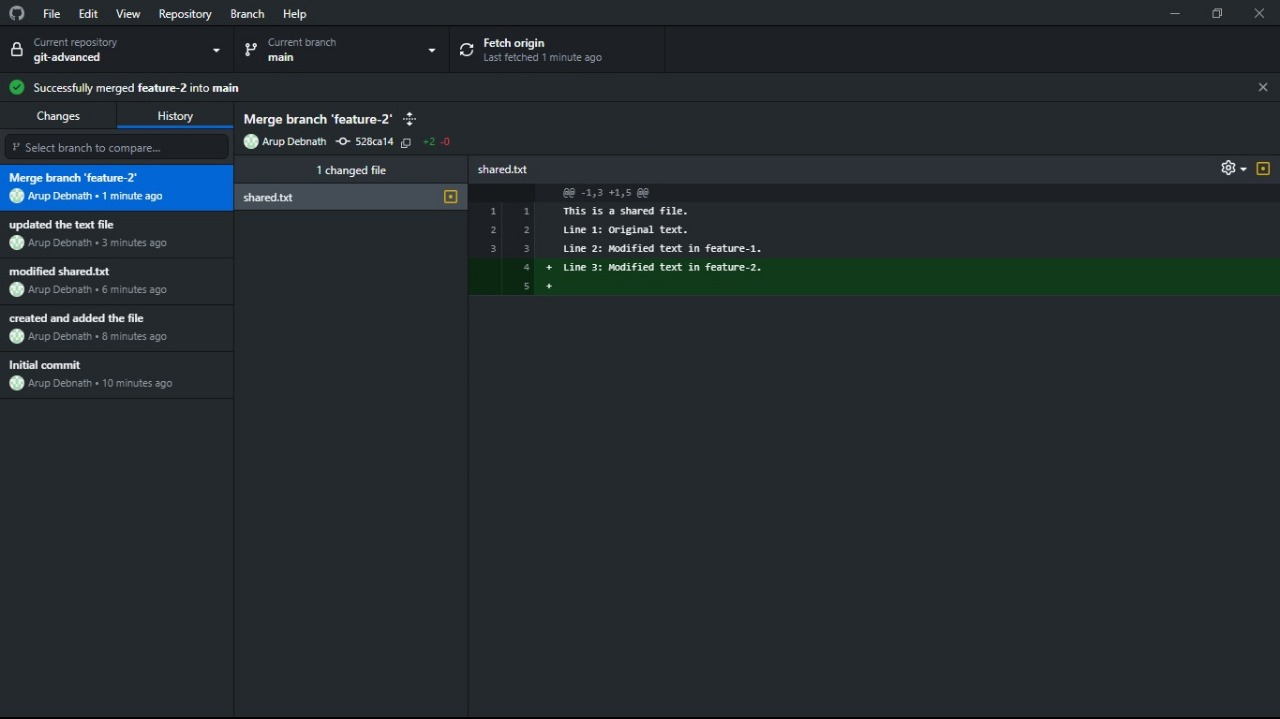
\includegraphics[width=12cm]{images/commit_history.jpeg}
    \end{center}
    
    \item A screenshot of the local machine showing the Git log and conflict resolution.
    \begin{center}
        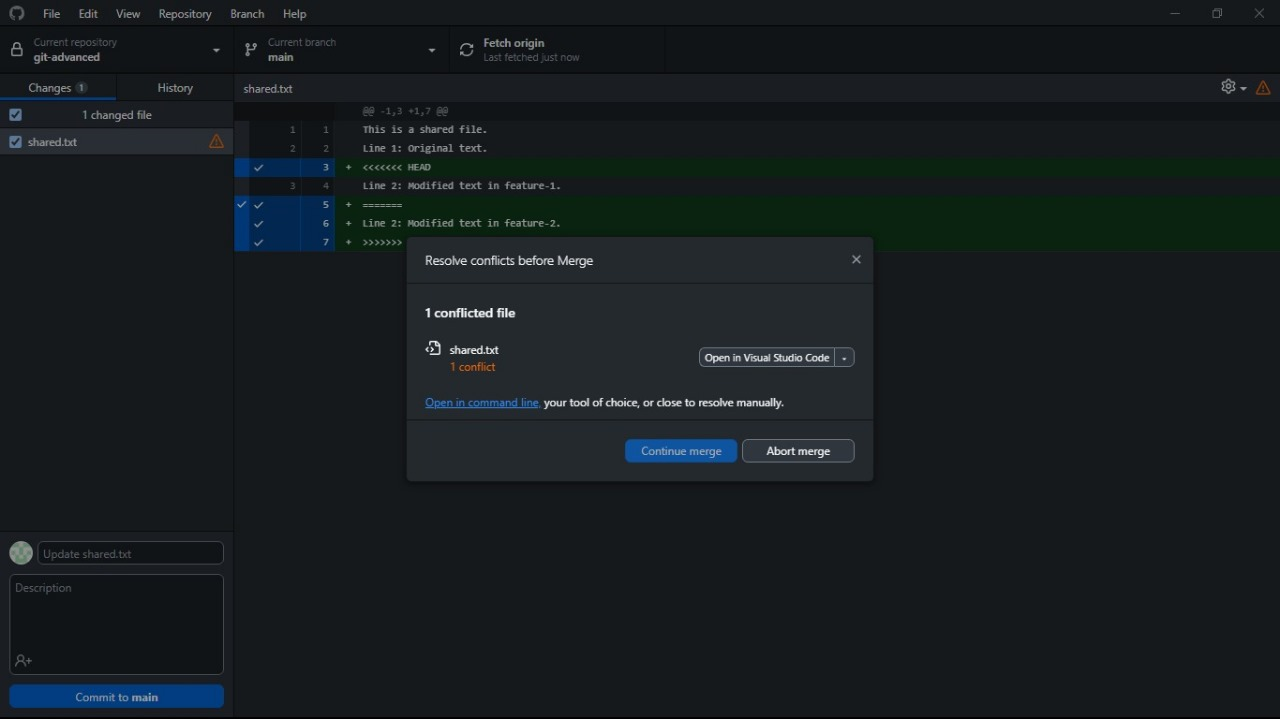
\includegraphics[width=12cm]{images/conflict.jpeg}
    \end{center}
    
    \begin{center}
        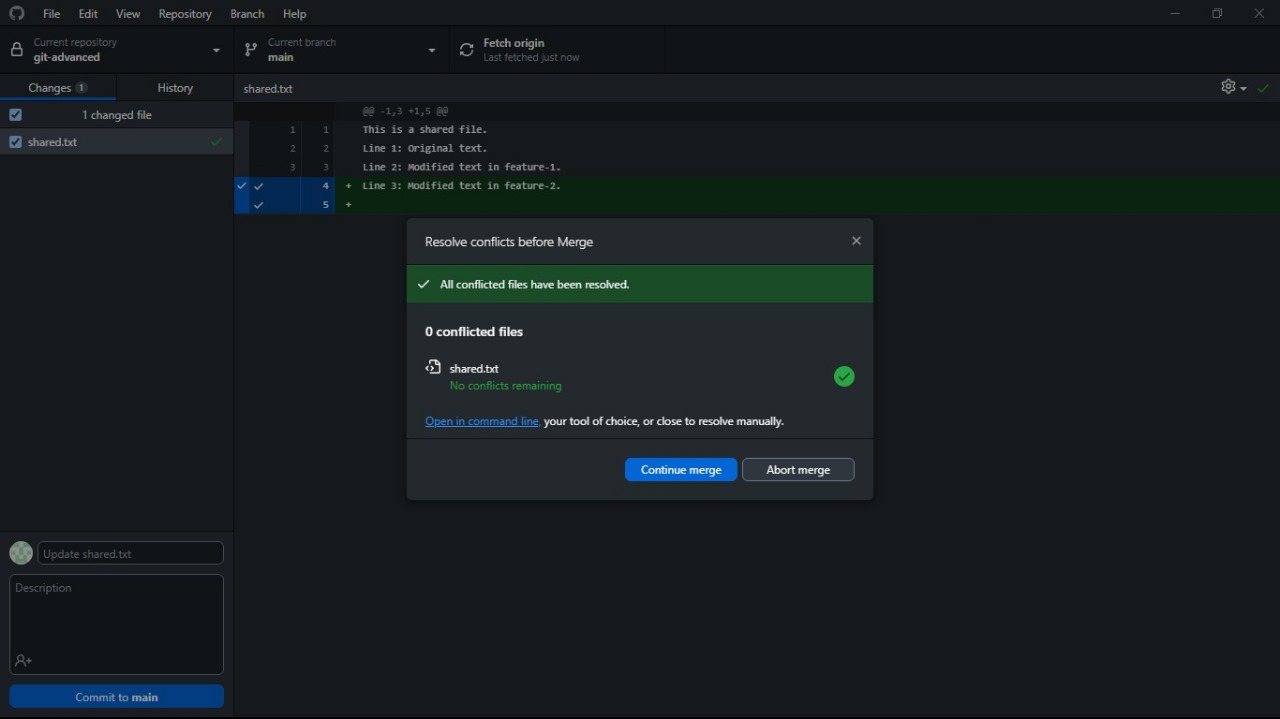
\includegraphics[width=12cm]{images/conflict_solved.jpeg}
    \end{center}
    
    \item A brief write-up of my experience with Git branching and merging.
\end{itemize}

\subsection{Conclusion}
This lab notebook entry documents the steps taken to successfully complete the assignment, showcasing the processes of branching, merging, and conflict resolution using the GitHub Desktop application.
